\documentclass{ximera}

\newcommand{\RR}{\mathbb R}
\renewcommand{\d}{\,d}
\newcommand{\dd}[2][]{\frac{d #1}{d #2}}
\renewcommand{\l}{\ell}
\newcommand{\ddx}{\frac{d}{dx}}
\newcommand{\dfn}{\textbf}
\newcommand{\eval}[1]{\bigg[ #1 \bigg]}


\author{Bart Snapp}


\begin{document}

\textbf{For problems 5--7,} consider the graph below of the vector-valued
function $\vec{p}(s)$. Additionally, suppose that $\vec{p}$ is
\textbf{parameterized by arc length}.
\begin{image}[4in]
    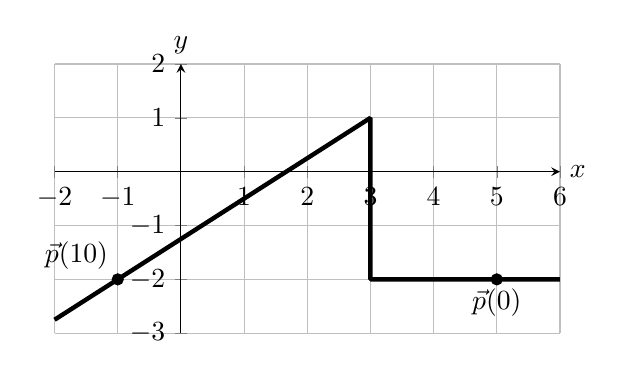
\begin{tikzpicture}
      \begin{axis}%
        [
	  xmin=-2,xmax=6,
          ymin=-3,ymax=2,
          xlabel=$x$,ylabel=$y$,
          axis lines=center,
          every axis y label/.style={at=(current axis.above origin),anchor=south},
          every axis x label/.style={at=(current axis.right of origin),anchor=west},
          clip=false,
	  grid =major,
          width=8cm,
          height=5cm,
          xtick={-2,-1,...,6},
          ytick={-3,-2,...,2},
	]
        \addplot[line join =bevel,black,ultra thick] coordinates{
          (-2,-2.75) (3,1) (3,-2) (6,-2)
        };
        \addplot[color=black,fill=black,only marks,mark=*] coordinates{(5,-2)};  %% closed hole
        \addplot[color=black,fill=black,only marks,mark=*] coordinates{(-1,-2)};  %% closed hole
        \node[black,below] at (axis cs: 5,-2) {$\vec{p}(0)$};
        \node[black,above left] at (axis cs: -1,-2) {$\vec{p}(10)$};
      \end{axis}
    \end{tikzpicture}
\end{image}

\begin{problem}
  Compute: $\int_0^{10} \vec{p}'(s)\dotp\vec{p}'(s)\d s$
  \begin{prompt}
    \[
    \int_0^{10} \vec{p}'(s)\dotp\vec{p}'(s)\d s =\answer{10}
    \]
  \end{prompt}
  \vspace{1in}
\end{problem}


\begin{problem}
  Compute: $\eval{\dd{s} \left(\vec{p}(s)\dotp\vec{p}(s)\right)}_{s=0}$
  \begin{prompt}
    \[
    \eval{\dd{s} \left(\vec{p}(s)\dotp\vec{p}(s)\right)}_{s=0} = \answer{-10}
    \]
  \end{prompt}
  \vspace{1in}
\end{problem}

\begin{problem}
  Compute: $\vec{p}(7.5)$
  \begin{prompt}
  \[
  \vec{p}(7.5) = \vector{\answer{1},\answer{-.5}}
  \]
  \end{prompt}
  \vspace{1in}
\end{problem}

\hrule

\begin{problem}
  \begin{prompt}
    Select statements that must be true:
  \end{prompt}
\begin{selectAll}
  \choice{The cross product of two unit vectors is always a unit vector.}
  \choice[correct]{A particle whose velocity vector is $\vec{v}(t) = \vector{2t,1/t,6t^2-1}$ could have position vector $\vec{p}(t) = \vector{t^2-1,\ln(t),2t^3-t+4}$.} 
  \choice{The plane $4x + 3y-z=0$ is perpendicular to the line $x=4t$, $y=3t$, $z=-t$.}
  \choice[correct]{If $\vec{v}$ and $\vec{w}$ are orthogonal, then $|\vec{v}+\vec{w}| = |\vec{v}-\vec{w}|$.}
  \choice{If $\vec{q}'(t) = \vector{e^t,\sin(t),3t^2}$ and $\vec{q}(0) = \vector{4,1,2}$, then $\vec{q}(t) = \vector{e^t+4,-\cos(t)+1,t^3+2}$.}
  \choice{None of the above.}
\end{selectAll}
\end{problem}



\end{document}
